% Original book diagram: fig:mc_exercise
% Book source: sections/appendices/appendixE.tex
% Original diagram authorship retained. Visual design: Ziad Mosalam.
\documentclass[11pt,border=8pt]{standalone}
\usepackage{amsmath,amssymb,graphicx,tikz}
\usetikzlibrary{arrows.meta,automata,positioning,calc,shapes.geometric,fit,backgrounds,patterns}
\newcommand{\vect}[1]{\mathbf{#1}}
\newcommand{\mat}[1]{\mathbf{#1}}
\newcommand{\Normal}{\mathcal{N}}
\newcommand{\prob}{p}
\newcommand{\E}{\mathbb{E}}
\newcommand{\Var}{\mathrm{Var}}
\newcommand{\Cov}{\mathrm{Cov}}
\newcommand{\CovP}{\mathbf{P}}
\newcommand{\Prob}{\mathbb{P}}
\setlength{\textwidth}{6.5in}
% Shared visual vocabulary for the book's original diagrams.
% Figures opt in explicitly, so unrelated text and existing additions are unchanged.
\definecolor{BookBlue}{HTML}{003262}
\definecolor{BookGold}{HTML}{B17A00}
\definecolor{BookTeal}{HTML}{247C86}
\definecolor{BookInk}{HTML}{30363B}
\definecolor{BookLight}{HTML}{E9EFF5}
\tikzset{
  book figure/.style={font=\small\rmfamily, color=BookBlue, text=BookInk,
    line width=0.8pt, >=Latex},
  book axis/.style={->, draw=BookInk, line width=0.6pt},
  book link/.style={->, draw=BookBlue, line width=0.8pt},
  book observation/.style={draw=BookGold, fill=BookGold!8},
  book state/.style={draw=BookBlue, fill=BookLight},
  book note/.style={font=\footnotesize\rmfamily, text=BookInk}
}

\begin{document}
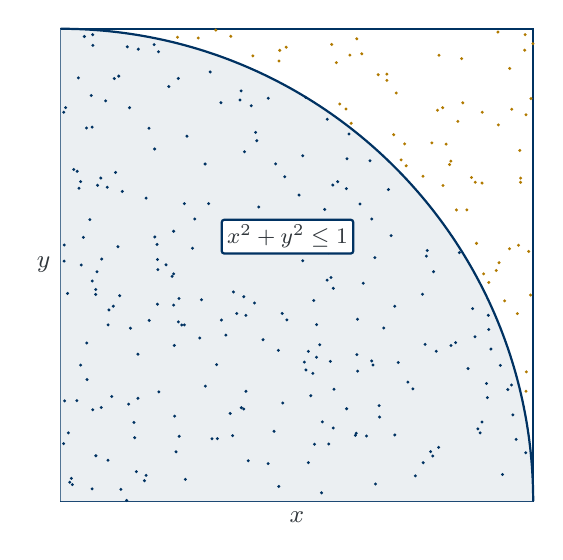
\begin{tikzpicture}[book figure, scale=6]
\pgfmathsetseed{42} % fixed seed so the figure is reproducible

% Draw the unit square
\draw[thick] (0,0) rectangle (1,1);

% Draw the quarter-circle (corrected)
\fill[BookBlue!8] (0,0) -- (1,0) arc (0:90:1) -- cycle;
\draw[BookBlue, thick] (1,0) arc (0:90:1);

% Axes labels
\node[below] at (0.5, 0) {$x$};
\node[left] at (0, 0.5) {$y$};

% Generate random points inside unit square
\foreach \i in {1,...,300} {
    \pgfmathsetmacro{\x}{rnd}
    \pgfmathsetmacro{\y}{rnd}
    \pgfmathsetmacro{\r}{\x*\x + \y*\y}
    \ifdim \r pt<1pt
        \fill[BookBlue] (\x,\y) circle (0.0035);
    \else
        \fill[BookGold] (\x,\y) circle (0.0035);
    \fi
}

% Label inside the quarter-circle
%%\node at (0.72,0.72) {\footnotesize $x^2 + y^2 \leq 1$};

\node[
    fill=white,
    draw=BookBlue,
    rounded corners=1pt,
    inner sep=2pt,
    font=\footnotesize
] at (0.48,0.56) {$x^2 + y^2 \leq 1$};

\end{tikzpicture}
\end{document}
